\chapter{Практические задания}

\begin{figure}[ht!]
	\centering{
		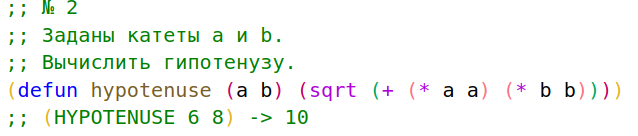
\includegraphics[width=0.8\textwidth]{img/2.png}
		\caption{Задание 2} }
\end{figure}


\begin{figure}[ht!]
	\centering{
		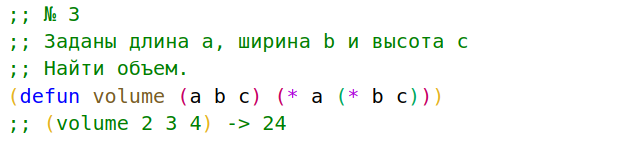
\includegraphics[width=0.8\textwidth]{img/3.png}
		\caption{Задание 3} }
\end{figure}


\begin{figure}[ht!]
	\centering{
		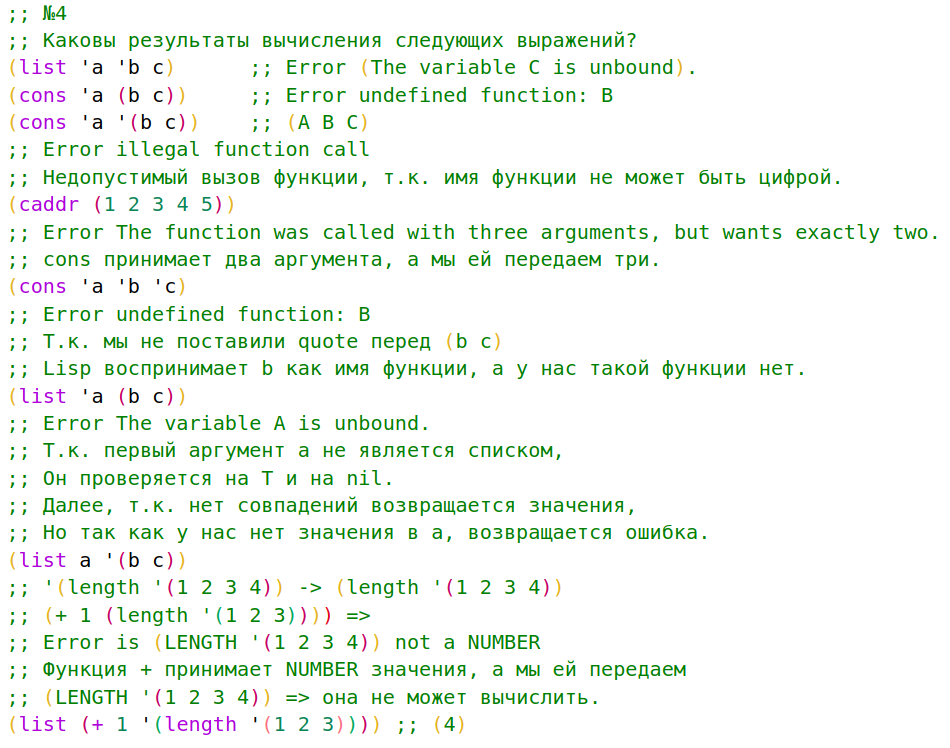
\includegraphics[width=0.8\textwidth]{img/4.png}
		\caption{Задание 4} }
\end{figure}

\begin{figure}[ht!]
	\centering{
		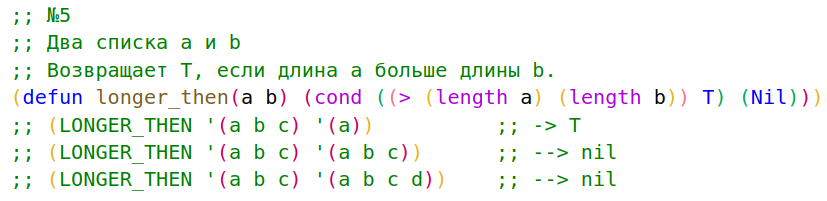
\includegraphics[width=0.8\textwidth]{img/5.png}
		\caption{Задание 5} }
\end{figure}

\begin{figure}[ht!]
	\centering{
		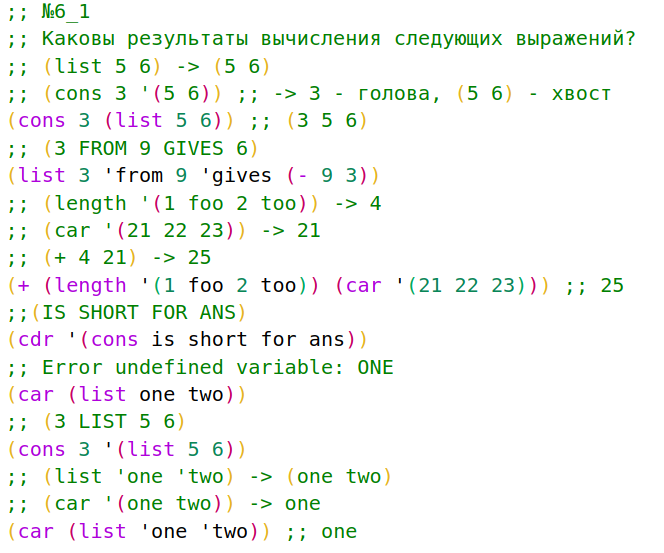
\includegraphics[width=0.8\textwidth]{img/6_1.png}
		\caption{Задание 6.1} }
\end{figure}

\begin{figure}[ht!]
	\centering{
		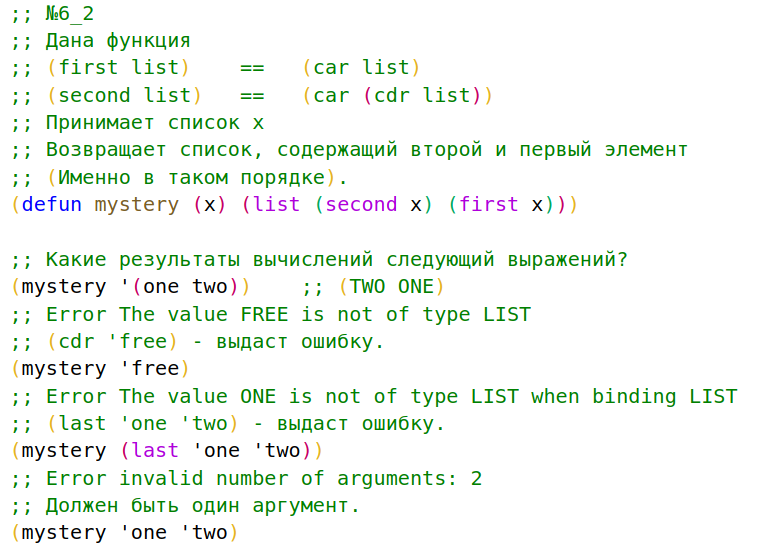
\includegraphics[width=0.8\textwidth]{img/6_2.png}
		\caption{Задание 6.2} }
\end{figure}

\chapter{Ответы на вопросы}

\section{Базис лиспа.}

\textbf{Базис} - минимальный набор средств для решения любой задачи.

Базис:

1) атомы и бинарные узлы;

2) atom, eq, cons, car, cdr, cond, quote, eval.

atom проверяет, является ли объект, переданный в качестве аргумента, атомом.

\begin{lstlisting}[language=Lisp]
(atom 'a) ;; t
(atom '(a b c)) ;; nil
\end{lstlisting}

eq проверяет идентичность двух символов.
\begin{lstlisting}[language=Lisp]
(eq 'a 'b) ;; nil
(eq 'a 'a) ;; t
\end{lstlisting}
	
cond - сокращение от англ. condition – условие. 
Не имеет фиксированного количества аргументов.
Каждый аргумент - это список, голова которого рассматривается как условие, 
и если оно истинно, то результатом будет хвост рассматриваемого списка.

\begin{lstlisting}
(cond ((eq 'A 'B) 'are_equal)
	 (T 'not_equal)) ;; NOT_EQUAL
\end{lstlisting}

eval - выполняет двойное вычисление своего аргумента.

\begin{lstlisting}
(eval (cons (quote car) (quote ('(A B))))) => A
		|---------(car '(A B))---------|

\end{lstlisting}

\section{Классификация функций.}

\begin{enumerate}
	\item Чистые математические функции - имеет фиксированное количество аргументов и один результат.
	\item Специальны функции - произвольное количество аргументов.
	\item Псевдофункции - создают эффект на экране.
	\item Рекурсивные функции.
	\item Функции с вариантными значениями, которые возвращают одно значение.
	\item Функции высших порядков - используются для построения синтаксически управляемых программ. %(абстракции языка)
\end{enumerate}

\textbf{Список} - динамическая структура данных, которая может быть
пустой или непустой. Если она не пустая, то состоит из двух элементов:

1. Головы - любая структура.

2. Хвоста - список.

Список представляет из себя заключенную в скобки
последовательность из атомов, разделенных пробелами, или списков.
Любой список является программой - его нужно вычислять.

\section{Как выполняются функции car и cdr}

car и cdr - базовые функции доступа к данным. 

\textbf{car} - принимает точечную пару или список и возвращает голову (первый элемент).
\textbf{cdr} - принимает точечную пару или список и возвращает хвост (все элементы, кроме первого).

\section{Отличие list и cons}

cons - имеет фиксированное количество аргументов (два). 
В случае, когда аргументами являются атомы создает точечную пару.
В случает, когда первый аргумент атом а второй список, атом становится головой,
а второй аргумент (список) становится хвостом. 
\begin{lstlisting}[language=Lisp]
(cons 'a 'b) 		 ;; (A . B)
(cons 'a '(a b c)) 	 ;; (A A B C)
(cons '(a c) '(b d)) ;;((A C) B D)
(cons 'a 'v 'd)  	 ;; Error (invalid number of arguments: 3)
\end{lstlisting}

\begin{figure}[ht!]
	\centering{
		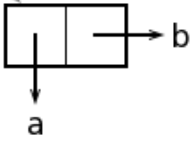
\includegraphics[width=0.25\textwidth]{img/img3.png}
		\caption{Результат cons.} }
\end{figure}

list - не имеет фиксированное количество аргументов. 
Создает список, у которого голова - это первый аргумент,
хвост - все остальные аргументы.
\begin{lstlisting}[language=Lisp]
(list 'a 'b) 				;; (A B)
(list 'a 'b 'v '(c d) 'd) 	;; (A B V (C D) D)
\end{lstlisting}

\begin{figure}[ht!]
	\centering{
		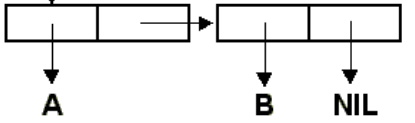
\includegraphics[width=0.5\textwidth]{img/img2.png}
		\caption{Результат list.} }
\end{figure}

\textbf{cons} - имеет фиксированное число аргументов и более экономный по памяти.

